\documentclass[11pt]{article}
\usepackage[sort]{natbib}
\usepackage{bm,amsmath,bbm,amsfonts,nicefrac,latexsym,amsmath,amsfonts,amsbsy,amscd,amsxtra,amsgen,amsopn,bbm,amsthm,amssymb,graphicx}
\usepackage{fancyhdr}
\usepackage[margin=1.0in]{geometry}
\usepackage[section]{placeins}
\bibliographystyle{abbrvnat}

\title{Thesis Introduction}
\author{Ewan Pinnington}

\newtheorem{theorem}{Theorem}[section]
\newtheorem*{defn}{Definition}


\begin{document}

\maketitle

\section{Notation}
List of symbols and meanings consistent throughout thesis.

\section{The global carbon cycle}

Carbon is one of the most abundant elements, making up around half of all living matter dry mass on Earth. The global carbon cycle describes the movement of carbon through the Earth system. In the Earth system large amounts of carbon are present in the oceans, atmosphere, land surface and crust. These stores of carbon are referred to as reservoirs or pools. The amount of carbon on Earth can be considered constant, as under terrestrial conditions it is not common to have nuclear transmutation. Therefore terrestrial processes using carbon must transfer it between the global carbon pools, this is referred to as a flux. In pre-industrial times these fluxes of carbon between different pools have remained approximately constant over long time scales REF.

The greenhouse gas effect describes the process by which radiatively active gases (CO2, water vapour, ozone, etc.) in the Earth's atmosphere contribute to the warming of the planet by absorbing long-wave radiation emitted from the Earth's surface and reradiating this absorbed energy in all directions, causing more warming below \citep{mitchell1989greenhouse}. The natural greenhouse gas effect raises the global mean surface temperature by 30K, making the Earth habitable for the many lifeforms upon it. The increase in atmospheric greenhouse gases since the industrial revolution due to anthropogenic activities has amplified the greenhouse effect and caused global warming. CO2 has been found to be the most important human-contributed compound to this warming \citep{Falkowski291}. In figure~\ref{fig:ipcc_fig6.1} we show a simplified schematic of the global carbon cycle taken from the Intergovernmental Panel on Climate Change (IPCC), in this schematic we can see the large rise in atmospheric CO2 since the industrial revolution with an increase of 240 Pg C.

As atmospheric CO2 levels have risen, natural sinks of CO2 (fluxes out of the atmosphere) have intensified with both the land surface and oceans absorbing more CO2 from the atmosphere. This can be see in figure~\ref{fig:ipcc_fig6.1}, with the the net ocean flux of CO2 to the atmosphere decreasing from an estimated +0.7~Pg~C~yr\(^{-1}\) to -2.3~Pg~C~yr\(^{-1}\) and the land surface flux of CO2 to the atmosphere decreasing from -1.7~Pg~C~yr\(^{-1}\) to -2.6~Pg~C~yr\(^{-1}\). More recent estimates from \citet{le2015global} indicate these sinks have further intensified with the ocean sink estimated to be 2.9 \(\pm 0.5\)~Pg~C~yr\(^{-1}\) and the land surface sink 4.1 \(\pm 0.9\)~Pg~C~yr\(^{-1}\) for the year 2014. It is vitally important to understand the response of these sinks of CO2 to climate change in the future. If either the oceans or land surface were to stop absorbing this same percentage of CO2 from the atmosphere we would see even more dramatic increases in atmospheric CO2 levels and thus see a much greater rate of global warming.  

Good paper to highlight the fact that the percentage of CO2 absorbed by the land surface has remained approximately constant with rising atmospheric CO2 levels??? Maybe just use IPCC fig 6.8?

In figure 6.1 and 6.8: Partitioning of fluxes important and hard (shown by error on estimates in fig 6.1). Land surface carbon uptake least understood mechanism in the global carbon cycle, ref IPCC. Will uptake remain the same under climate change.

Human emissions of CO2 have perturbed the global C cycle and caused a large continual increase in atmospheric CO2 levels.

Look at papers recommended on Flux Course, some good ones to reference???

\begin{figure}[ht]
    \centering
    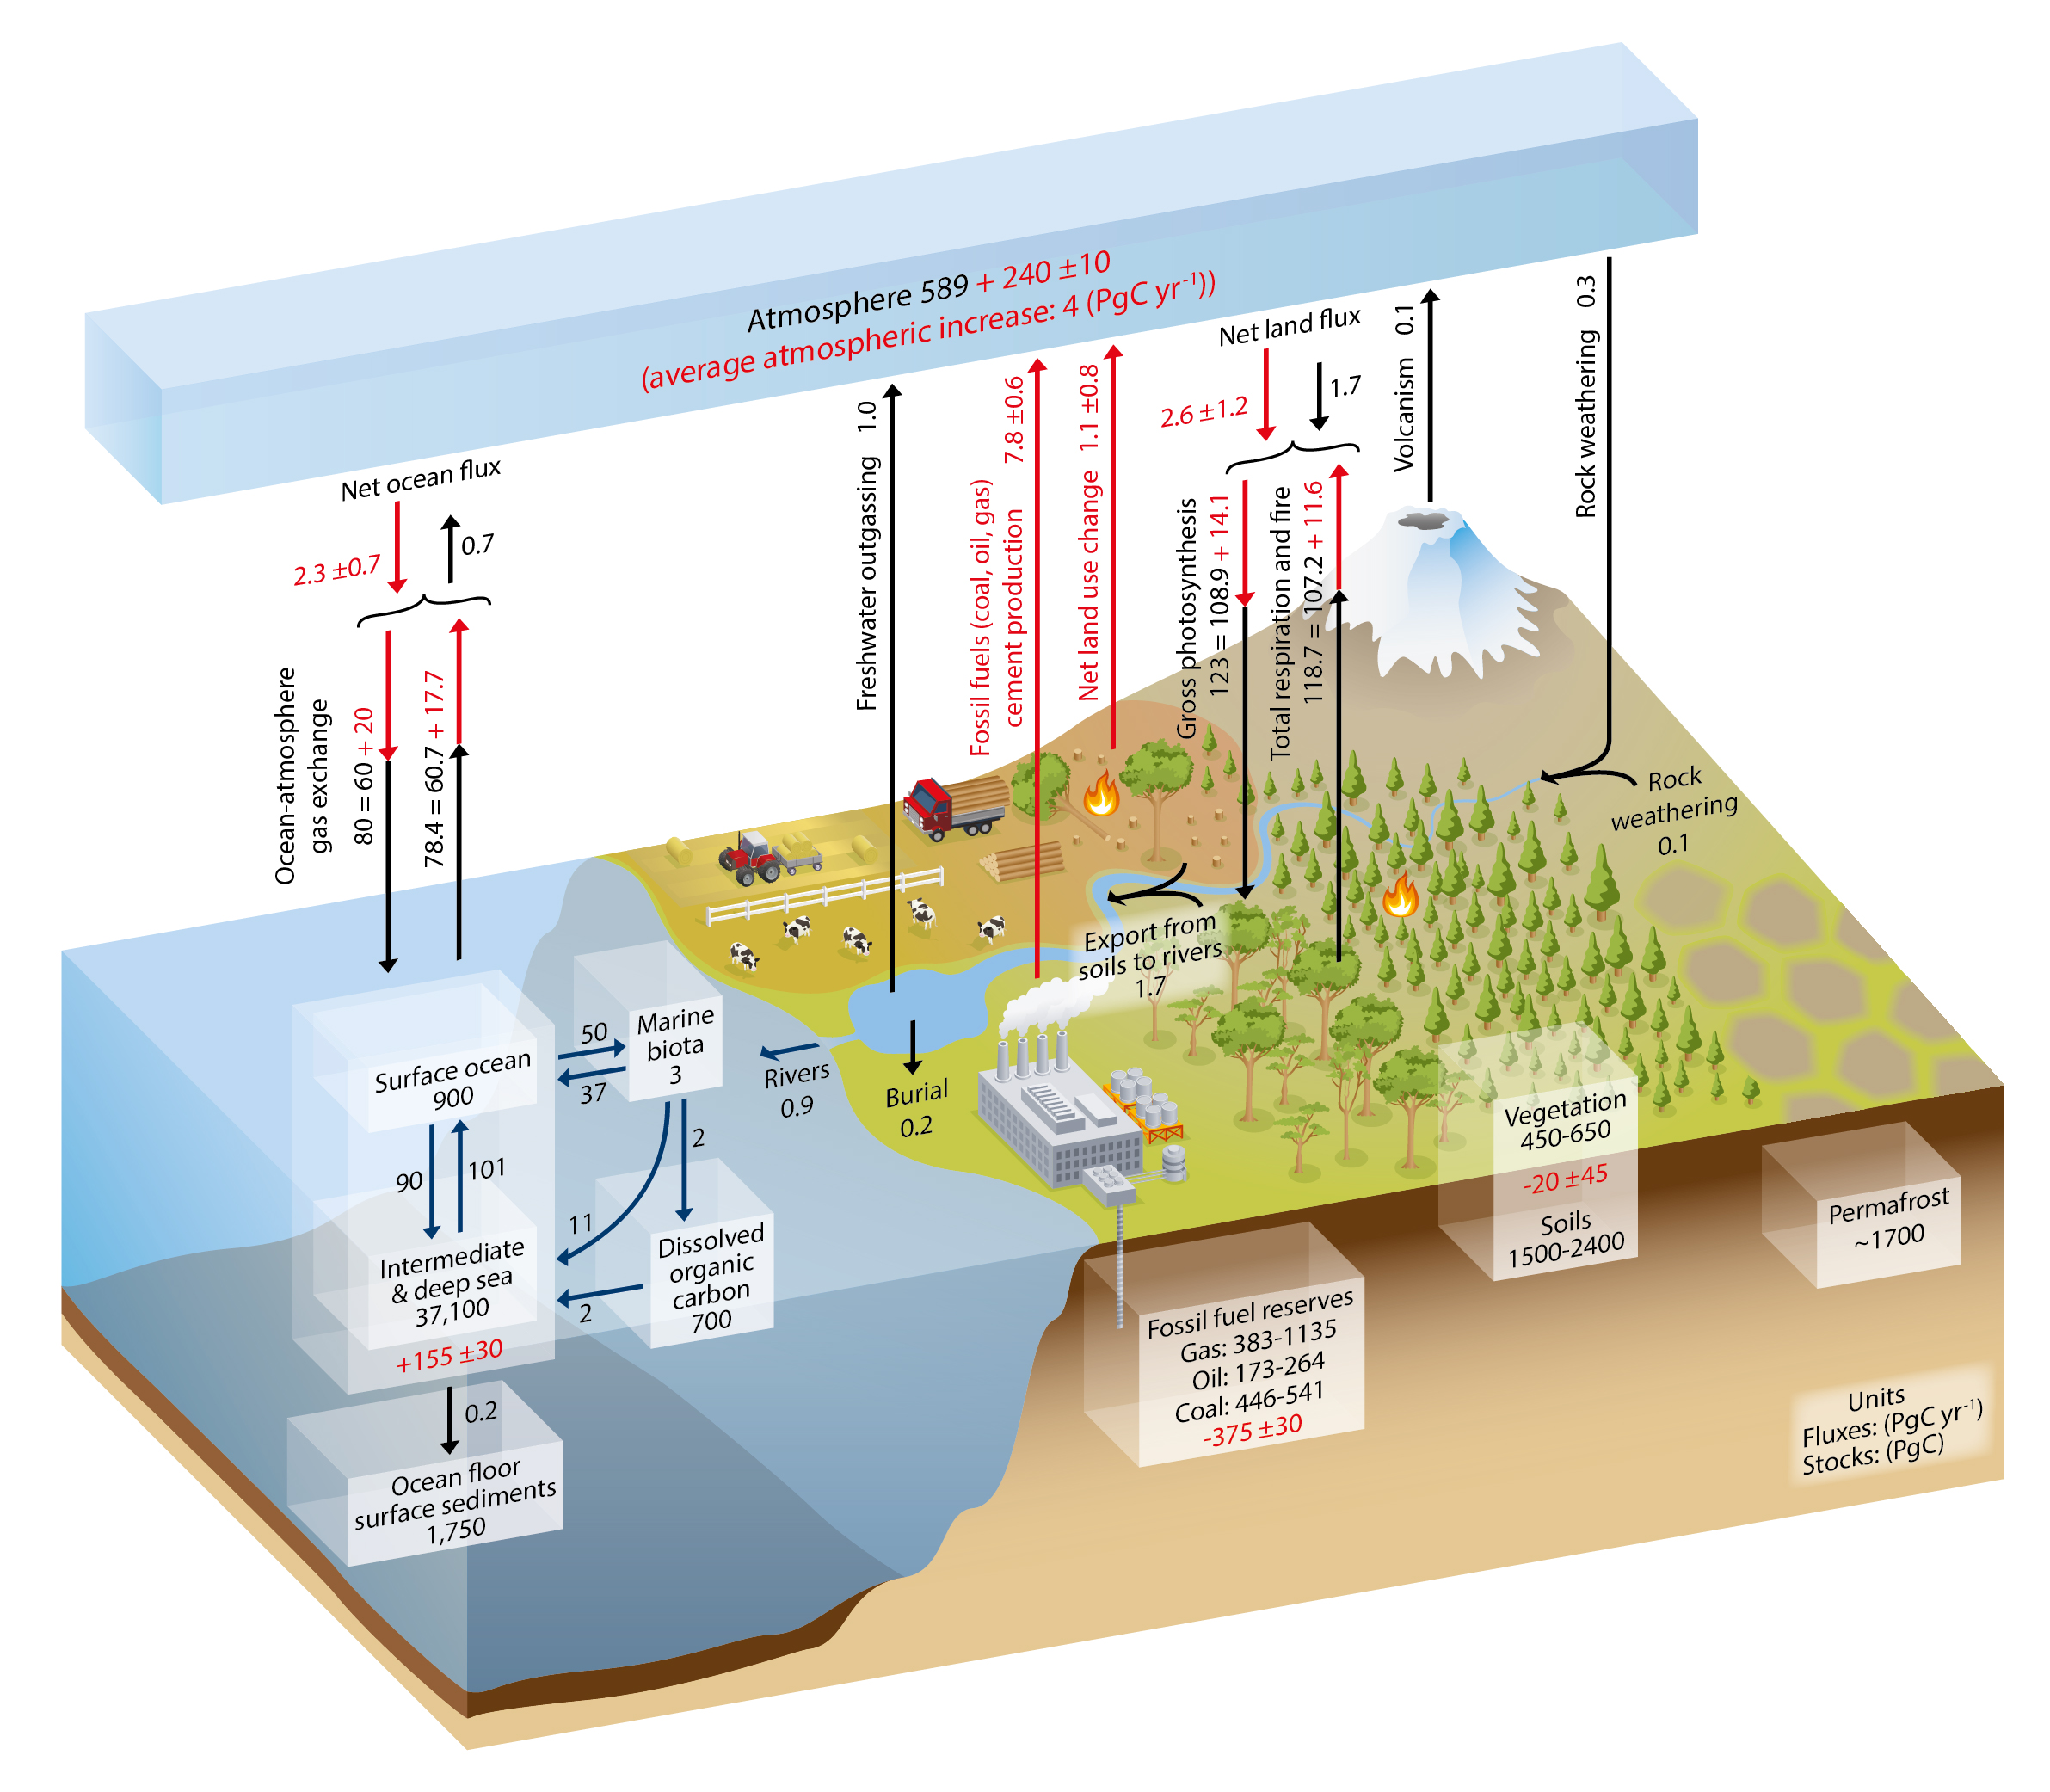
\includegraphics[width=0.7\textwidth]{ipcc_fig6_1.jpg}
    \caption{Global carbon cycle simplified schematic \citep{ciais2014carbon}. Black numbers and arrows represent reservoir mass and exchange fluxes estimated for the time prior to the industrial era (\(\sim\)~1750). Red numbers and arrows represent annual fluxes average over the 2000-2009 time period. Red numbers in the reservoirs indicate the cumulative change of carbon over the industrial period (1750-2011).}
    \label{fig:ipcc_fig6.1}
\end{figure}

\begin{figure}[ht]
    \centering
    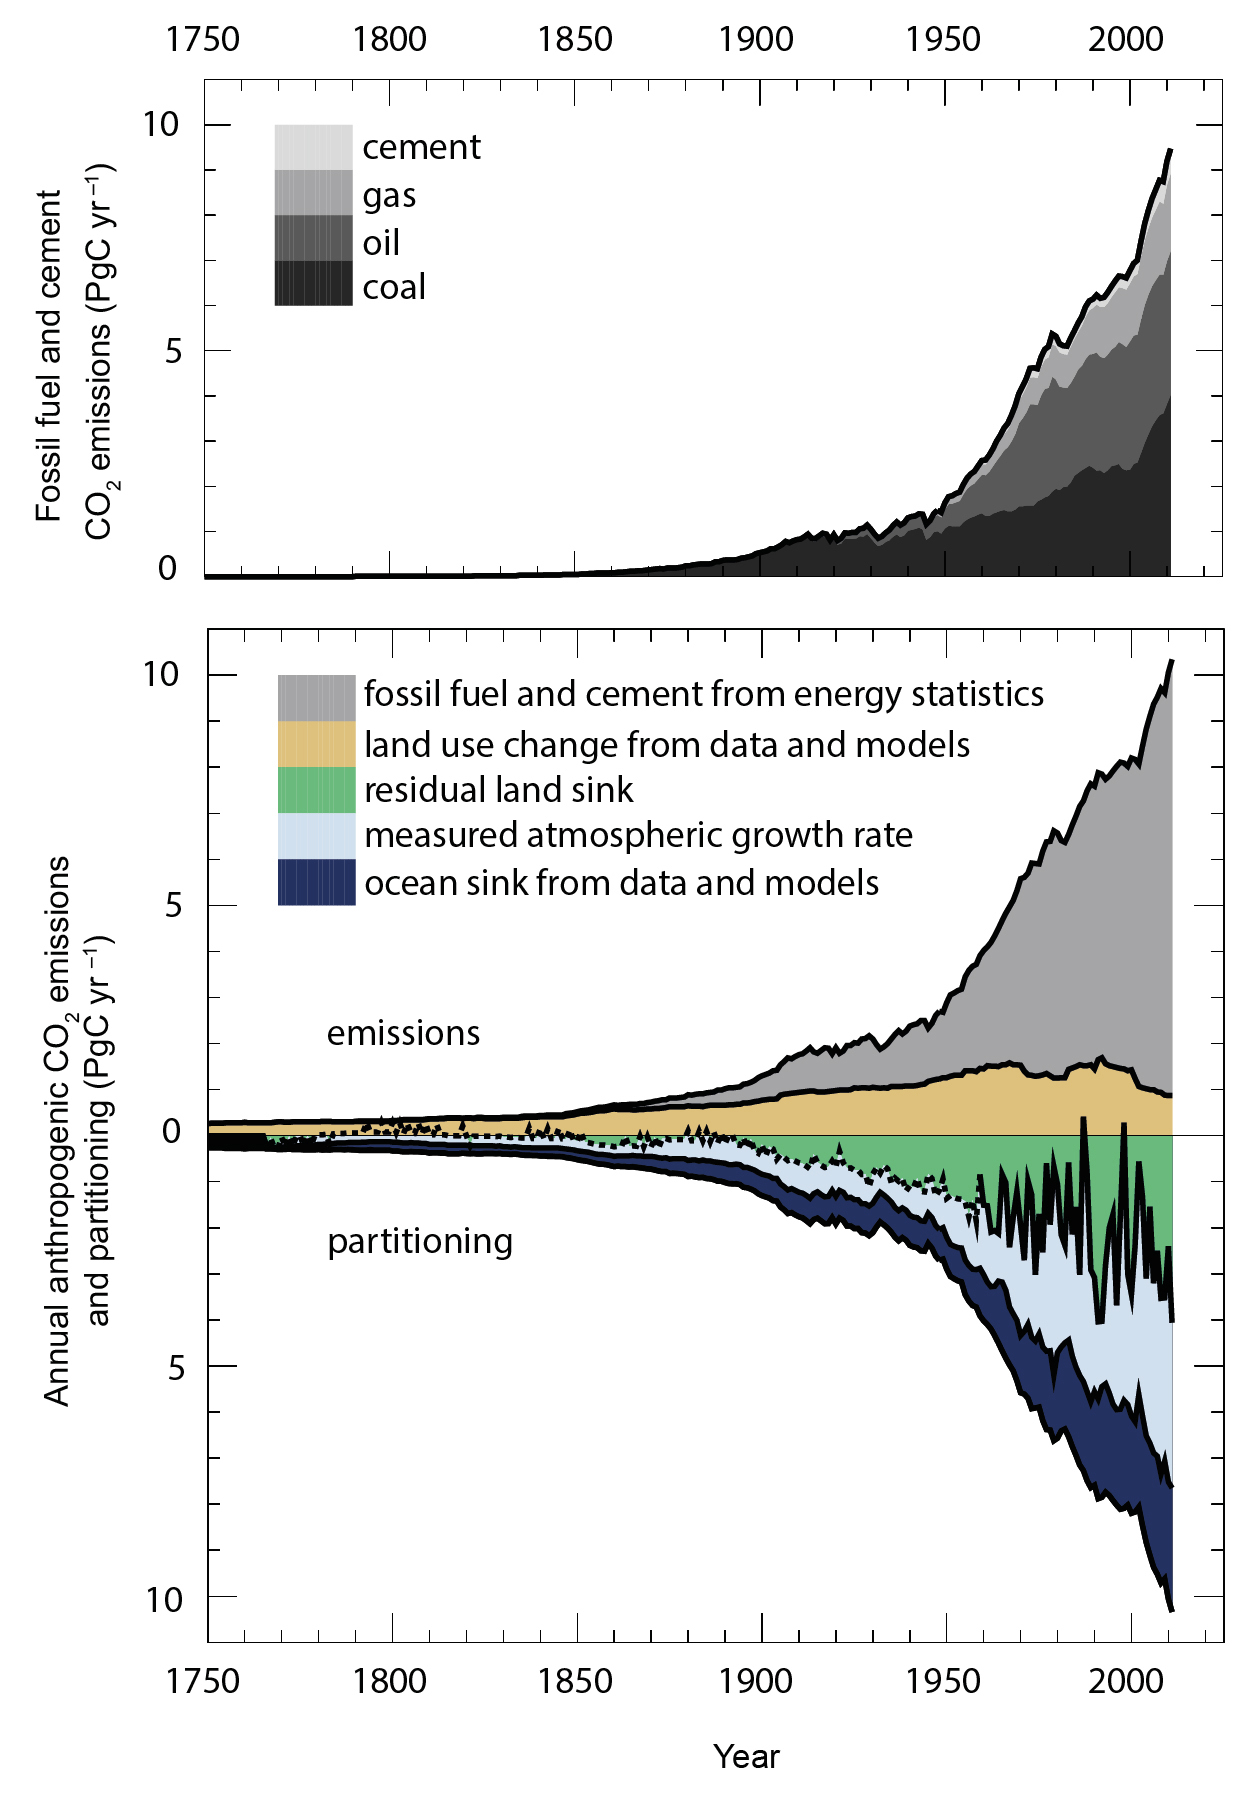
\includegraphics[width=0.7\textwidth]{ipcc_fig6_8.jpg}
    \caption{Annual anthropogenic CO2 emissions and their partitioning amoung the atmosphere, land and ocean from 1750 to 2011  \citep{ciais2014carbon}.}
    \label{fig:ipcc_fig6.8}
\end{figure}

IPCC figure 6.1 and 6.8: Partitioning of fluxes important and hard (shown by error on estimates in fig 6.1). Land surface carbon uptake least understood mechanism in the global carbon cycle, ref IPCC. Will uptake remain the same under climate change.

\citet{1748-9326-7-2-024002} Have shown that global warming is highly sensitive to land carbon cycle processes and highlighted the need to improve understanding of land surface carbon uptake and its response to climate change. 

\section{The role of models}

\begin{figure}[ht]
    \centering
    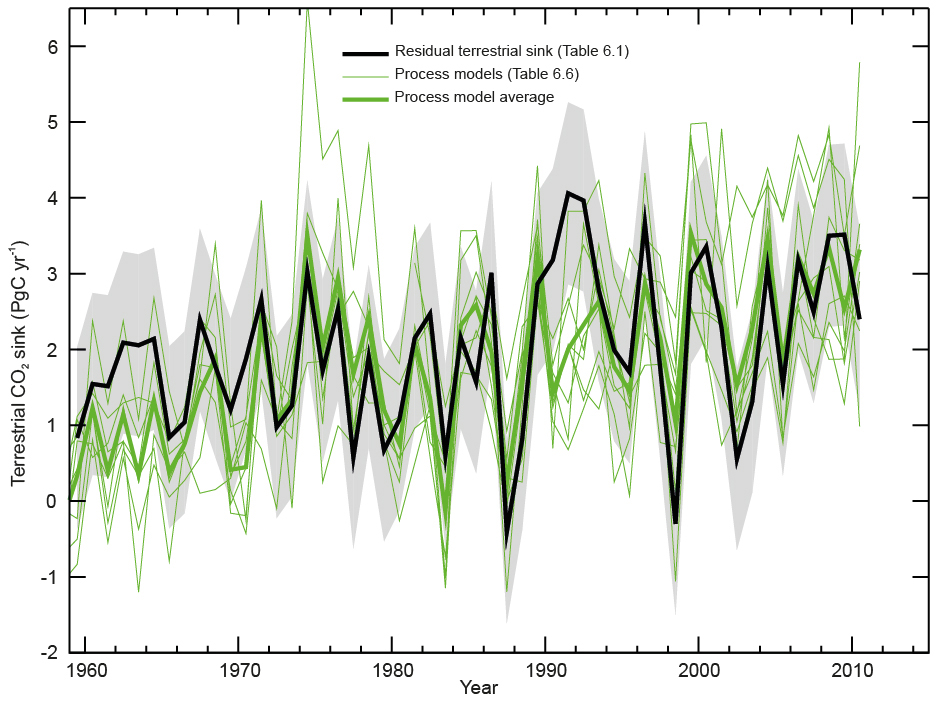
\includegraphics[width=0.9\textwidth]{ipcc_fig6_16.jpg}
    \caption{Modelled land sink \citep{ciais2014carbon}.}
    \label{fig:ipcc_fig6.16}
\end{figure}

IPCC figure 6.16 and section 6.3.2.6.6: Contribution of models to understanding the terrestrial carbon cycle. Reference every DALEC paper.

\section{Eddy covariance and other observations}

Baldocchi paper: Many observations of forest carbon flux made worldwide.

\section{Data assimilation}

Role of DA in NWP improving forecast skill. 


\bibliography{../PhD}{}
\end{document}